\documentclass[tikz,border=3pt]{standalone}
\usepackage[T1]{fontenc}
\usepackage{helvet}
\usetikzlibrary{arrows.meta,positioning}
\begin{document}
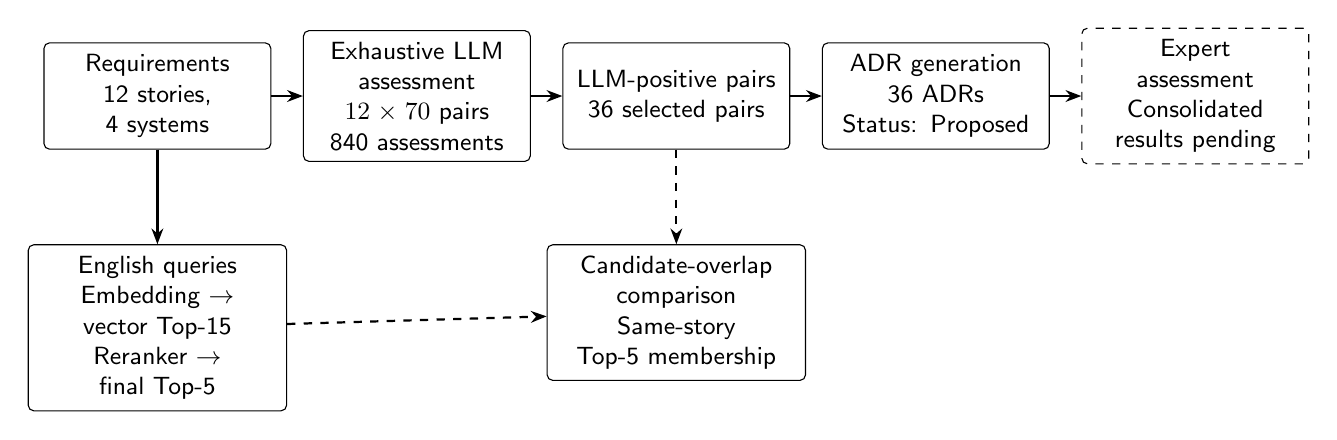
\begin{tikzpicture}[
  font=\sffamily\small,
  stage/.style={draw,rounded corners=2pt,align=center,text width=2.6cm,
                minimum height=1.35cm,inner sep=4pt},
  flow/.style={-{Stealth[length=2mm]},thick},
  compare/.style={flow,dashed}
]
\node[stage] (requirements) {Requirements\\12 stories, 4 systems};
\node[stage,right=4mm of requirements] (assessment) {Exhaustive LLM\\assessment\\$12 \times 70$ pairs\\840 assessments};
\node[stage,right=4mm of assessment] (selected) {LLM-positive pairs\\36 selected pairs};
\node[stage,right=4mm of selected] (adrs) {ADR generation\\36 ADRs\\Status: Proposed};
\node[stage,dashed,right=4mm of adrs] (experts) {Expert\\assessment\\Consolidated\\results pending};
\draw[flow] (requirements) -- (assessment);
\draw[flow] (assessment) -- (selected);
\draw[flow] (selected) -- (adrs);
\draw[flow] (adrs) -- (experts);
\node[stage,below=12mm of requirements,text width=3cm] (rag) {English queries\\Embedding $\to$ vector Top-15\\Reranker $\to$ final Top-5};
\node[stage,below=12mm of selected,text width=3cm] (overlap) {Candidate-overlap comparison\\Same-story\\Top-5 membership};
\draw[flow] (requirements) -- (rag);
\draw[compare] (rag) -- (overlap);
\draw[compare] (selected) -- (overlap);
\end{tikzpicture}
\end{document}
